%
	為了改善室內定位的覆蓋率以及定位的精確度,本研究利用建置虛擬相片的方法來增加照片的取樣範圍,及過濾無法擷取照片特徵的
不適角度。定位實驗與平面 SIFT 影像定位方法做比較,利用數據及圖表做分析探討。定位實驗分成兩個實驗環境來驗證定位方法所改善的數據:
(1)景物單一且特徵固定的實驗環境、(2)一般室內定位的環境。

	在景物單一且特徵固定的實驗情境下,我們驗證每個固定距離內 SIFT 所涵蓋的特徵點數量作比較,藉由增加
與物體的固定距離算出固定距離內的平均定位誤差,在誤差容忍範圍與平面照片影像定位覆蓋率作比較。在特徵固定的環境下根據
實驗情境與實驗方法說明改善的成果,再把定位方法放建築在一般實際的室內環境中作比較,最後呈現出改善的平均定位誤差與增加環
境所能定位的覆蓋率。為了完成這些實驗,所用到的電腦設備為 Intel CORE i5(2.0GHz CPU、8GB RAM),顯卡為了能夠使
用 CUDA 平行運算加速,所採用的是 nVIDIA 520MX 的顯示晶片,以及拍攝環境所使用的 Kinect 紅外線深度攝影機。

%1. Controlled Enviornment 
\section{景物單一情境下定位結果分析}

% 控制環境實驗目的與成效描述
	建立可以控制的實驗環境主要目的為在景物單一且可以控制的特徵點數環境下與一般平面影像定位做比較,藉由實驗驗證出更好的定位覆蓋率
與更小的平均定位誤差。在根據有限特徵數量的環境下,將待定位的照片依距離增加,生成出格狀的位置的照片定位點,每個定位點前後
都有固定的間距距離,利用這些待定位照片,分別進行三種實驗方法比較結果:
							
\begin{enumerate}
  \item 特徵點數量分布分析
  \item 間距定位誤差分布分析
  \item 定位精準度覆蓋率以及平均定位誤差
\end{enumerate}

\begin{table}[htbp]
  \centering
  \caption{控制環境實驗參數設定}
    \begin{tabular}{rrr}
    \toprule
    實驗設定 :  & 控制環境 1 & 控制環境 2 \\
    \midrule
    待定位照片數量 : & 45 張  & 54 張 \\
    間距寬度 : & 0.5m & 0.5m \\
    間距長度 : & 0.75m & 0.5m \\
    \bottomrule
    \end{tabular}%
  \label{table:Controlled EV parameters}%
\end{table}%

一開始建置景物單一情境環境,我們將這些定位照片分布在 4公尺 X 5公尺的環境大小內,
而景物的分布在 1.5公尺 X 0.7公尺的大小範圍內, Kinect 攝影機放置在距離景物 0.5公尺前的地方,利用 Kinect 攝影機拍照取得深度照片與待定位的照片,待定位照片與虛擬照片解析度皆為
640 x 480。在表中\ref{table:Controlled EV parameters}所示,在兩個控制環境的實驗中,利用不同的定位環境、不同的間距以及不同待定位圖片的數量來做實驗比較。
		
\subsection{特徵點數量趨勢}

\begin{figure}
\begin{center}
  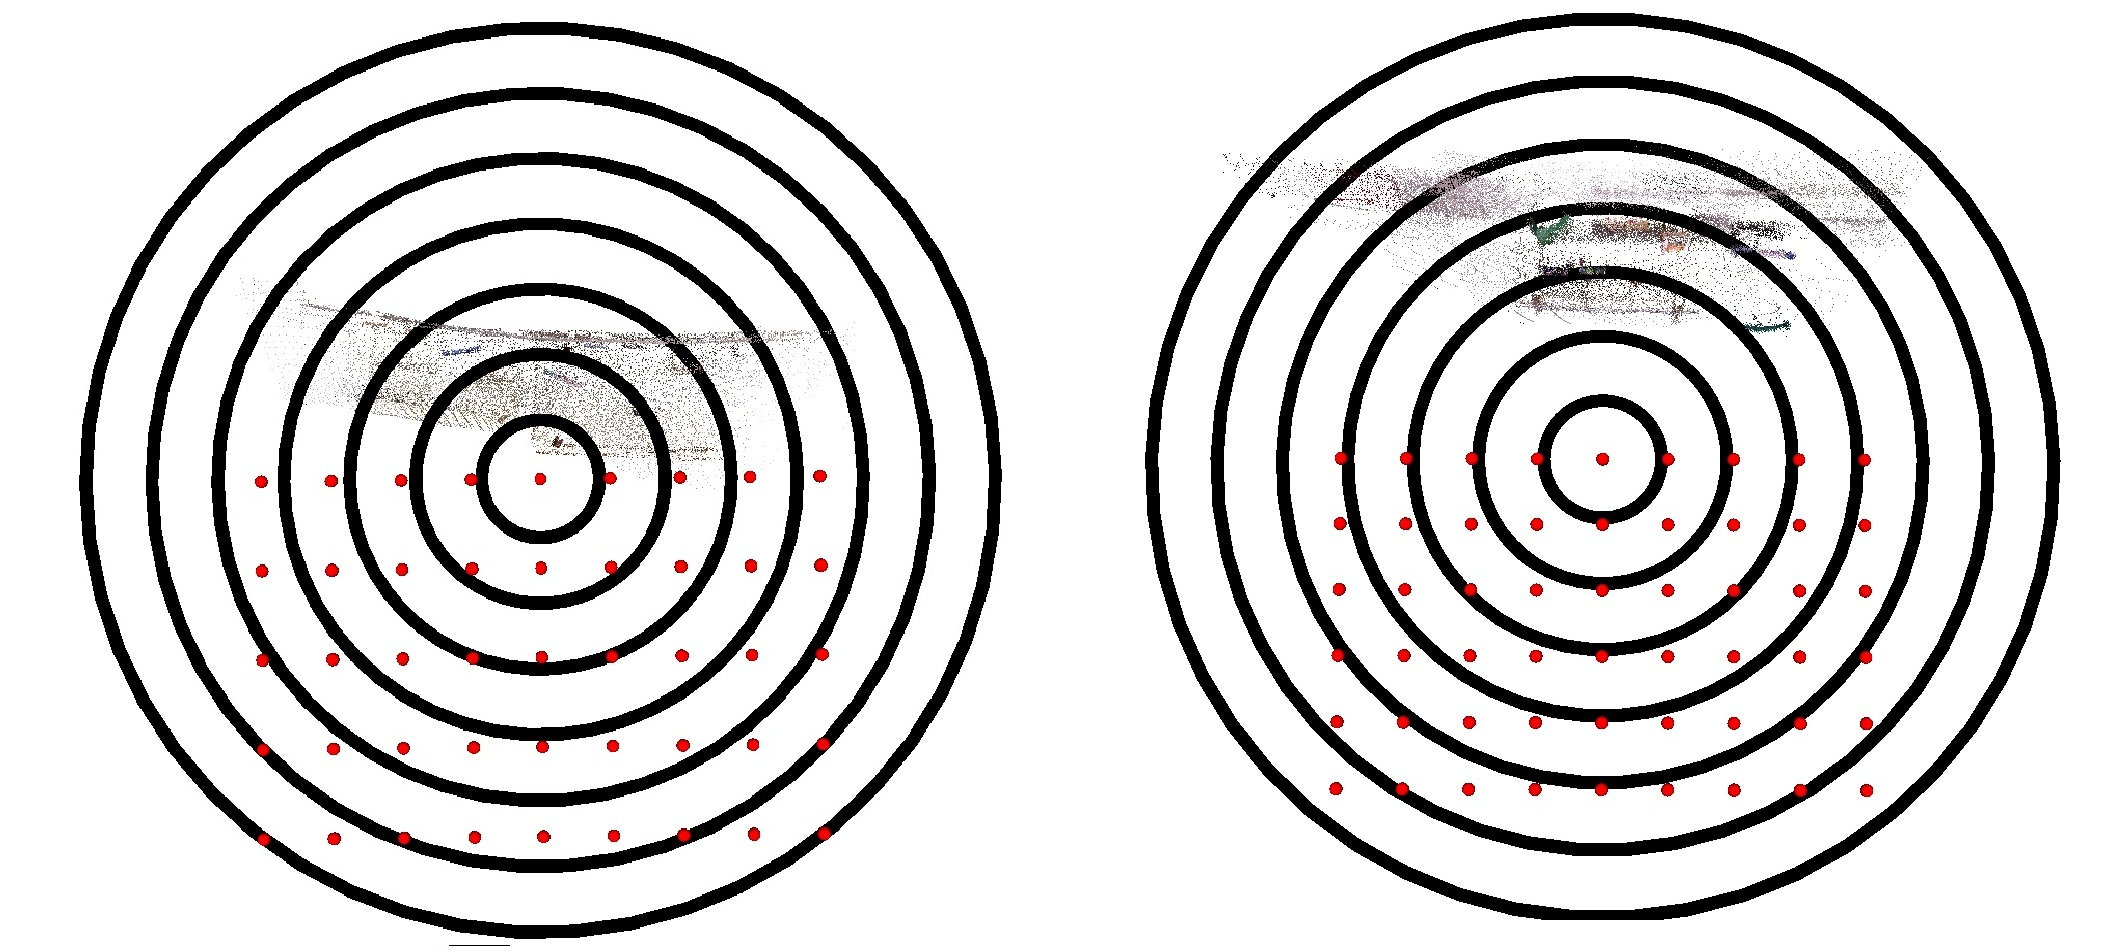
\includegraphics[width=1.0\textwidth]{figures/CoverDisk.jpg}
  \caption{依照同心圓的覆蓋算出每個半徑內的每張圖的特徵點平均數,左.控制環境 1 右.控制環境 2}
  \label{fig:CoverDisk}
\end{center}
\end{figure}

\begin{figure}
	\begin{center}
    \subfigure[控制環境 1.特徵點平均數量比較]{\label{fig:CoverDisk_Descriptor1}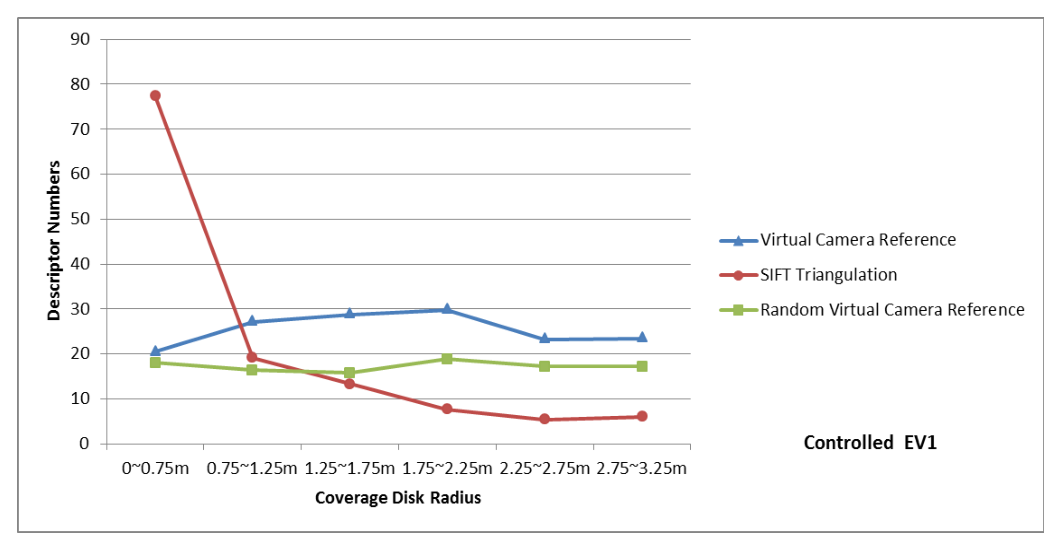
\includegraphics[width=0.9\columnwidth]{figures/Controlled_EV1_DescriptorNum.eps}}
    \subfigure[控制環境 2.特徵點平均數量比較]{\label{fig:CoverDisk_Descriptor2}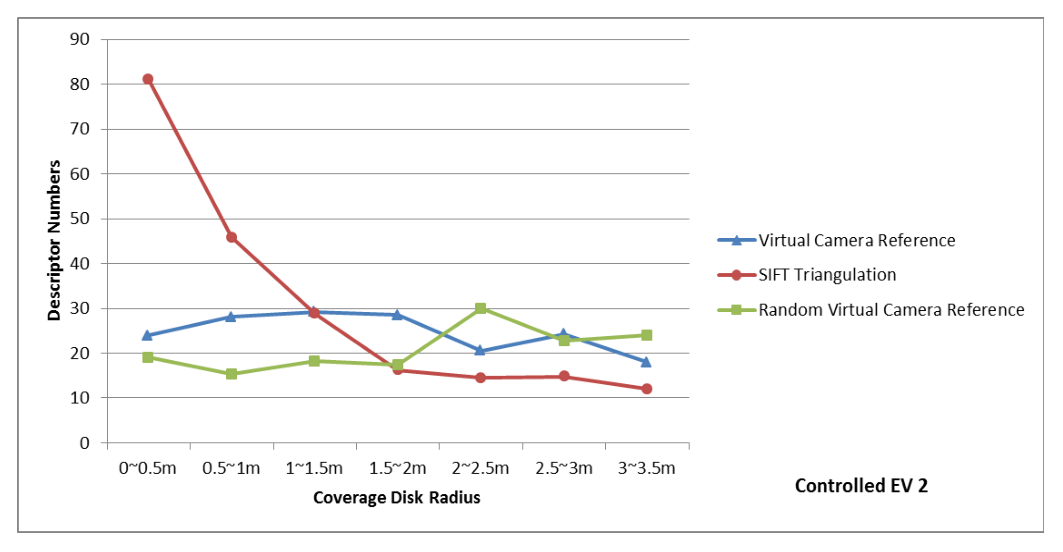
\includegraphics[width=0.9\columnwidth]{figures/Controlled_EV2_DescriptorNum.eps}}
	\end{center}
  \caption{特徵點數量趨勢圖,根據距離增加看出特徵點分布的數量差異情形}
  \label{fig:CoverDisk_DescriptorNum}	
\end{figure}

	這個實驗目的是要看出根據景物的距離增加與特徵點數量的關係圖,實驗的作法是先在待定位圖片的第一排中間設為圓心,如圖
\ref{fig:CoverDisk}所示。根據這個圓心將圓的半徑以間距距離的長度增加,像是控制環境1.中根據每個間距距離增加0.75m,控制環境2.中                                                                               
每個間距距離增加0.5m,依據每個圓之間所能覆蓋的特徵點位置做特徵點數量的總和並算出平均值,藉由圖中的趨勢看出特徵點數量的變化。下面根據
圖\ref{fig:CoverDisk_DescriptorNum}分析距離長度與特徵點數量作圖表分析。

	根據圖\ref{fig:CoverDisk_DescriptorNum}所示,
特徵點的數量變化,以虛擬影像格狀分布的數量為最穩定且平均數量較高的狀態,圖\ref{fig:CoverDisk_Descriptor1}在間距0.75 m的分布情形下,都有其對應的特徵點可供參考,
反觀SIFT影像特徵雖然在一開始可以找到多數的特徵點,但是隨著距離增加,數量逐步遞減,最後只有些許的特徵可以找出。圖\ref{fig:CoverDisk_Descriptor2}在間距0.5 m的分
布情形下,格狀分布的優勢較不明顯,SIFT平面影像特徵點數量趨勢下滑也趨於緩慢。

	圖\ref{fig:CoverDisk_Descriptor1}與圖\ref{fig:CoverDisk_Descriptor2}分析得出間距距離大,對格狀分布與隨機分布的影響差異越大,其中這些數量上的差異會影響之
後間距定位的成果。尤其在圖\ref{fig:CoverDisk_Descriptor1}間距0.75 m下的數量差異最為明顯,而格狀的虛擬相機分布其特徵點數量呈穩定的趨勢,比起隨機分布更能運在室內定
位上,改進資料蒐集不完全的問題。
	
\begin{figure}
	\begin{center}
    \subfigure[控制環境 1.間距定位平均誤差比較]{\label{fig:Distance_Error1}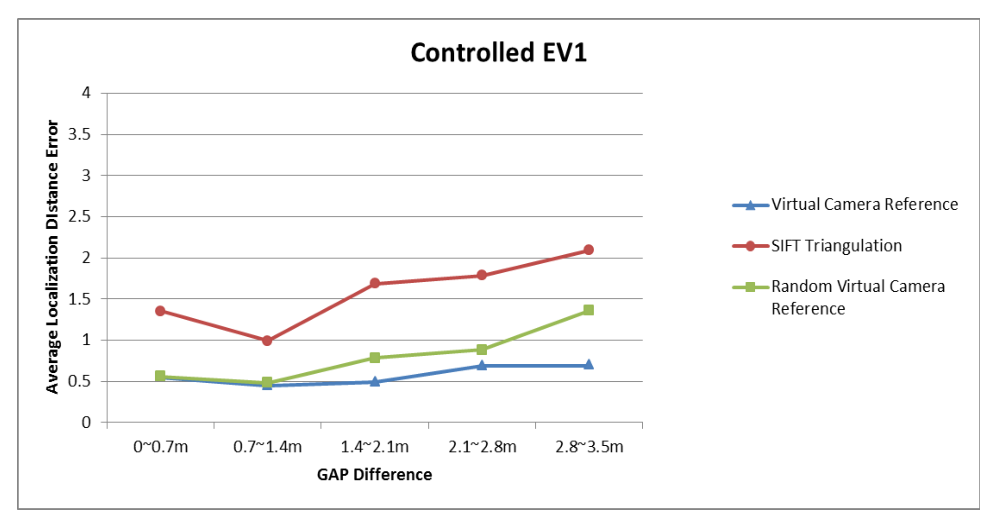
\includegraphics[width=0.9\columnwidth]{figures/Controlled_EV1_Localization_Distance_Error.eps}}
    \subfigure[控制環境 2.間距定位平均誤差比較]{\label{fig:Distance_Error2}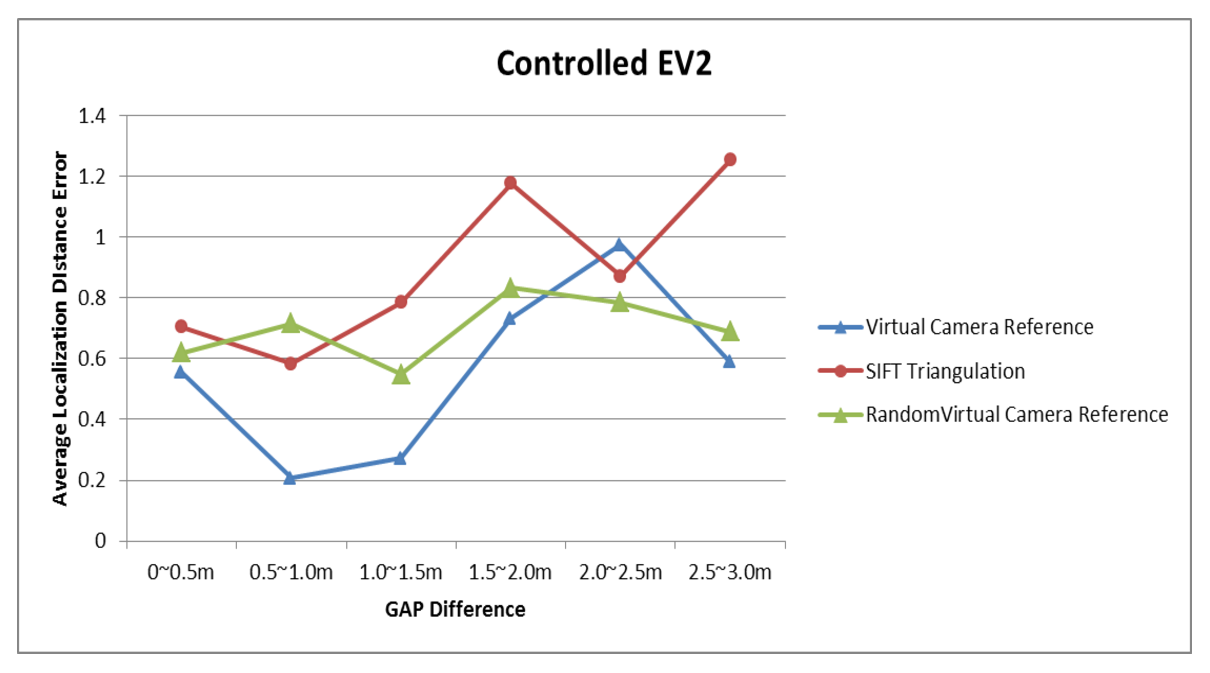
\includegraphics[width=0.9\columnwidth]{figures/Controlled_EV2_Localization_Distance_Error.eps}}
	\end{center}
  \caption{間距定位平均誤差趨勢圖,以每一橫排的待定位圖片平均誤差做計算,看出距離增加對定位誤差是否有影響}
  \label{fig:Localization_Distance_Error}	
\end{figure}	
	
\subsection{間距定位誤差趨勢}	
	
	以圖\ref{fig:Localization_Distance_Error}可看出,以每一橫排的待定位圖片的平均誤差分布,根據每一個不同的間距,虛擬相機圖片定
位比一般相機所做出的影像定位誤差都有改善,尤其以圖\ref{fig:Distance_Error1}格狀分布的3D虛擬影像改善最為明顯。根據我們的方法,我們想要模擬在不同的角度及位置產生3D虛
擬影像,比起一般的傳統影像有更多可以做特徵點匹配的相片可供使用。

傳統的平面影像定位所做出的資料庫中,對於景物比較遠的照片並沒有資訊提供,只
能利用拘限在景物較近的照片可供定位,但是少許的特徵點使得定位誤差更加放大,所以照圖中趨勢來看,距離一增加,定位誤差就會加大。但是在3D虛擬影
像不會因為距離的增加,導致定位誤差增加。除了3D虛擬影像可以增加更多可以被匹配的相片以外,好的虛擬相機分布,也可以產生更多的特徵點可以被匹配
。以隨機分布與格狀分布來說,隨機分布的3D虛擬相片雖然有改善,但沒有比格狀分布的虛擬相片改善來的明顯。

在我們的方法中,我們定位會參考照相機所
在的位置,所以定位的位置都會在相機位置的附近,隨機分布可能會造成某些區域的相機分布過於集中,某些相機卻又過於分散的情況發生。所以在隨機虛擬
相機分布的定位其實就跟平面相機分布的定位分布差不多,差別在於相片角度會避開障礙物,但不會均勻分布在環境中;格狀平均分布的攝影機位置,就會均
於分布在環境內,而對於影像特徵點匹配上比隨機分布來的更有幫助。


\subsection{定位精準度覆蓋率以及平均定位誤差分布情況}	
	
\begin{figure}
	\begin{center}
	\rotatebox{90}{
	\subfigure[控制環境 1.]{\label{fig:Controlled_EV1_Result}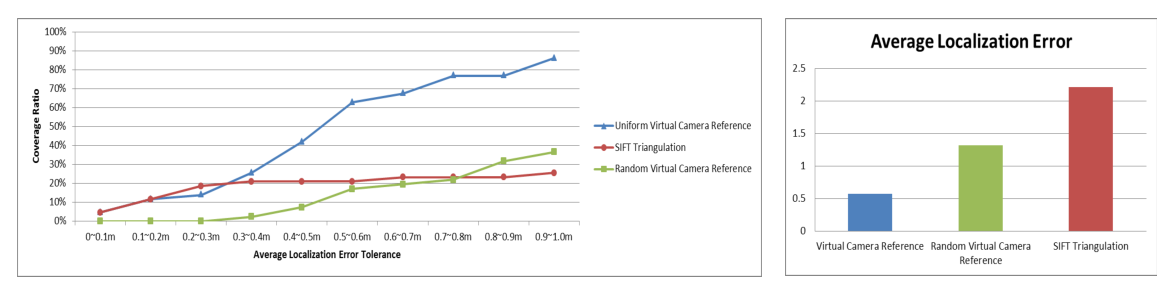
\includegraphics[width=1.2\columnwidth]{figures/Controlled_EV1_Result.eps}}
	}
	\rotatebox{90}{
	\subfigure[控制環境 2.]{\label{fig:Controlled_EV2_Result}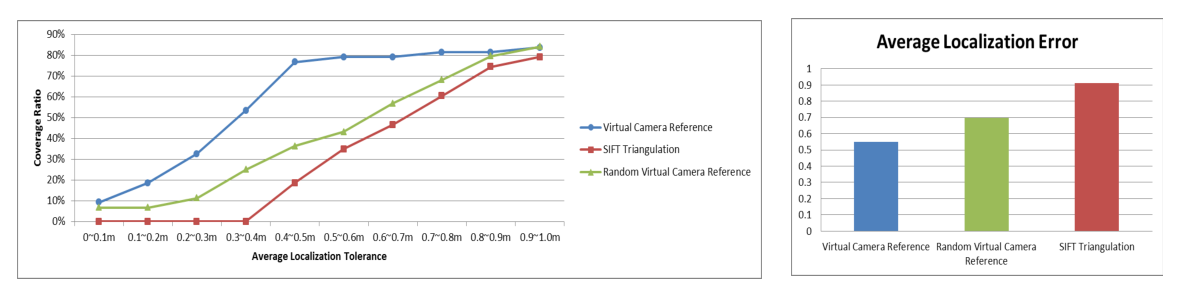
\includegraphics[width=1.2\columnwidth]{figures/Controlled_EV2_Result.eps}}
	}
	%\subfigure[平均定位誤差]{\label{fig:Controlled_AVG_Error}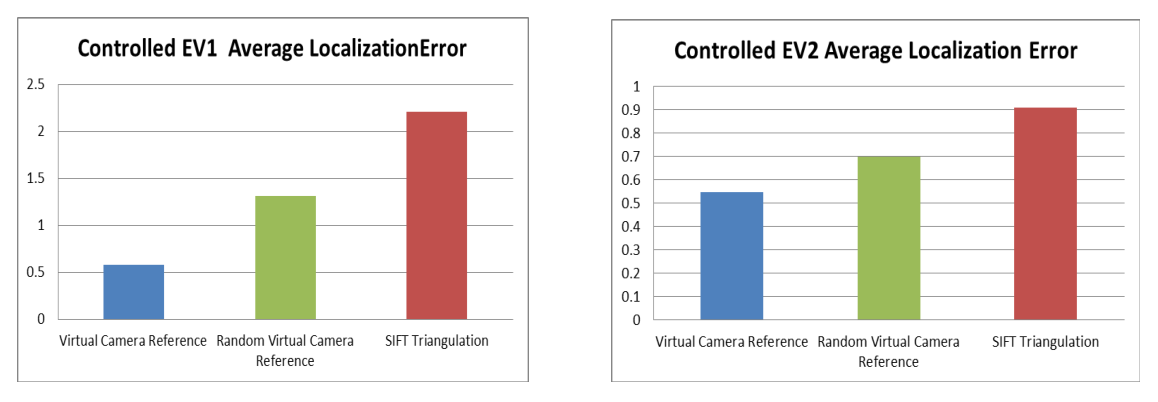
\includegraphics[width=1.0\columnwidth]{figures/Controlled_Average_Result.eps}}
	\end{center}
  \caption{控制環境下定位精準度覆蓋率以及平均定位誤差成果分析,(a),(b)圖為誤差容忍範圍下,可定位成功的覆蓋率分布情形}
  \label{fig:Controlled_EV_Result}	
\end{figure}	

\begin{figure}
\begin{center}
  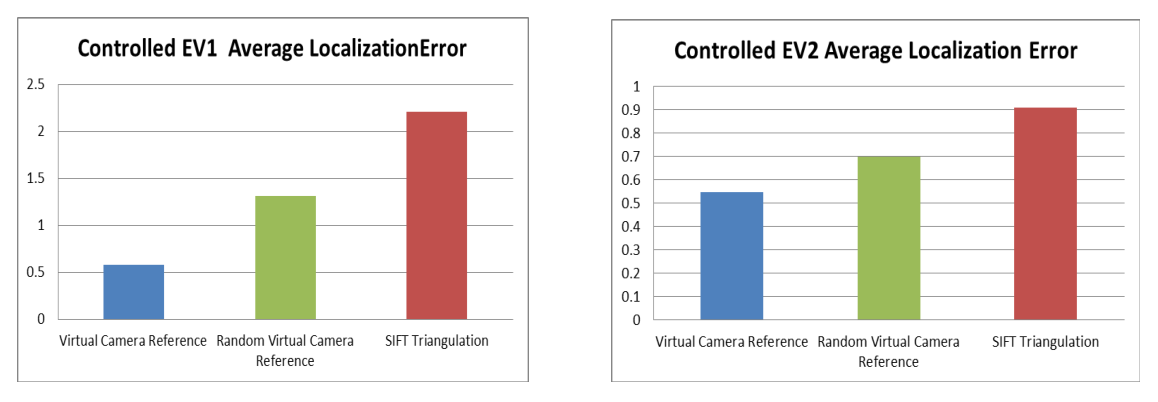
\includegraphics[width=1.0\textwidth]{figures/Controlled_Average_Result.eps}
  \caption{控制環境下定位平均誤差}
  \label{fig:Controlled_AVG_Error}
\end{center}
\end{figure}

	研究發現與景物的距離越遠在3D虛擬影像定位並不會影響誤差,整體來看,對定位的覆蓋率也有一定的提升。根據圖\ref{fig:Controlled_EV1_Result}與圖\ref{fig:Controlled_EV2_Result}
所示,在格狀分布
的3D虛擬相機定位在誤差0.5 m左右有超過$60\%$的覆蓋率,但隨機分布的虛擬相機以及2D平面影像定位坐落在$20\% \sim 30\%$左右上下,表示相機的分
布影響定位結果的好壞,這也是我們讓照相機格狀分布平均的原因。藉由均勻取得的定位資訊,改善影像蒐集中容易遺漏的邊緣及死角,確保在定位時,能保留定位
資料的完整性,避免相機分布不均導致資料遺漏的情形發生。

回到圖\ref{fig:CoverDisk_Descriptor1}來看,在1.75 m以後的隨機虛擬相
片所找出特徵點平均數量比起格狀分布虛擬相片所找出的特徵點數量少上許多,而在圖\ref{fig:Distance_Error1}來看,每個間距的定位平均誤差,
格狀分布都比隨機分布的誤差好上許多。所以當以誤差在0.6 m以內的覆蓋率來說,隨機分布的虛擬相片並沒有產生比較好的定位覆蓋率,但以格狀分布的
虛擬相片定位覆蓋率與2D影像定位覆蓋率相比,結果好上許多。

這說明虛擬相機分布的位置,影響了虛擬相片的品質,
平均定位誤差平均定位的誤差以格狀的虛擬影像為物誤差為最低,2D影像定位的誤差為最高,改善了整體定
位的平均誤差。最後以圖\ref{fig:Controlled_AVG_Error}來看,格狀分布的虛擬影像定位平均誤差皆
為最小,在單一景物的定位環境實驗下,研究方法能夠對定位平均誤差與覆蓋率作改善,也證實景物不會因相機
距離增加導致誤差發生。最後在一般室內環境下根據定位誤差與覆蓋率作實驗分析。

%2. Indoor Localization
\section{一般室內環境定位實驗}

	在控制環境下,改善了定位的覆蓋率與精準度,在這章節將在一般室內環境下進行定位測試。我們將室內定位環境分成兩種情境:(1)
居家客廳 ,(2) 居家廚房與 ,分別在這兩種環境下進行定位實驗。在一般室內定位主要進行定位覆蓋率與定位平均誤差測試。
	
	在室內定位的情況下,拍攝待定位照片的方法依據環境情況而定。待定位照片拍攝方法是依照人能夠活動的範圍作依據,在這些區域進行
格點分布拍攝,如圖\ref{fig:Indoor_EV1_query}與圖\ref{fig:Indoor_EV2_query}所示。每張待定位圖片的間距距離為0.5公尺,
照片數量根據環境大小而定,平均在30張上下。虛擬照片依據間距距離,取出不同數量的虛擬相機。因為考量不同環境的景物分布,每組相機位置
分別拍攝兩種不同的角度,最後根據虛擬相機拍攝出的照片作影像定位。除了與2D影像定位方法做比較之外,分別測試在不同虛擬照片資料數量的
定位情形。
		
\begin{table}[htbp]
  \centering
  \caption{室內定位環境大小分布}
    \begin{tabular}{rrr}
    \toprule
    實驗設定 :  & 客廳 & 廚房 \\
    \midrule
    待定位照片數量 : & 35 張  & 30 張 \\
    間距距離 : & 0.5m & 0.5m \\
    環境長度 : & 3.8m & 4.1m \\
    環境寬度 : & 4.1m & 3.2m \\
    \bottomrule
    \end{tabular}%
  \label{table:Indoor EV parameters}%
\end{table}%
	
	
	表2.2 記錄了不同室內定位環境的設定,分別在不同環境下進行實驗,每個環境的虛擬相機位置均採用格狀分布。圖\ref{fig:Indoor_EV_and_Query}
記錄當時點雲環境的建置以及待定位照片的位置分布。點雲的建置是利用Kinect環繞室內環境四周所拍攝,再利用這些拍攝的圖片,當作平面2D影像定位
所需的影像資料庫。接下來分別以不同虛擬相機照片的數量與平面2D影像做實驗比較分析。
	
\subsection{定位覆蓋率與定位平均誤差分析比較}

\begin{figure}
	\begin{center}
	\subfigure[定位環境 1.客廳環境]{\label{fig:Indoor_EV1}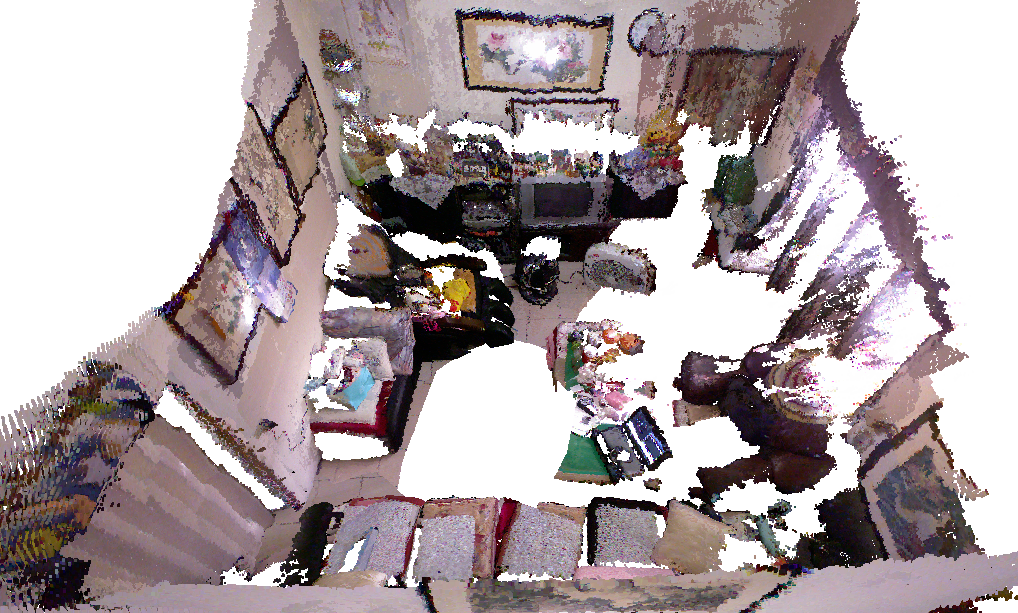
\includegraphics[width=0.45\columnwidth]{figures/snapshot00.jpg}}
	\subfigure[定位環境 2.廚房環境]{\label{fig:Indoor_EV1}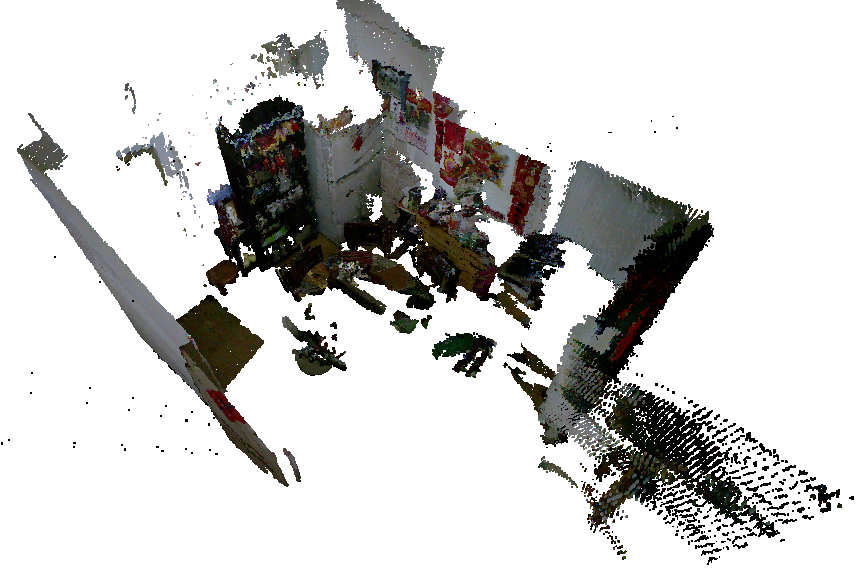
\includegraphics[width=0.45\columnwidth]{figures/snapshot01.jpg}}
    \subfigure[定位環境 1.客廳 待定位照片分布位置]{\label{fig:Indoor_EV1_query}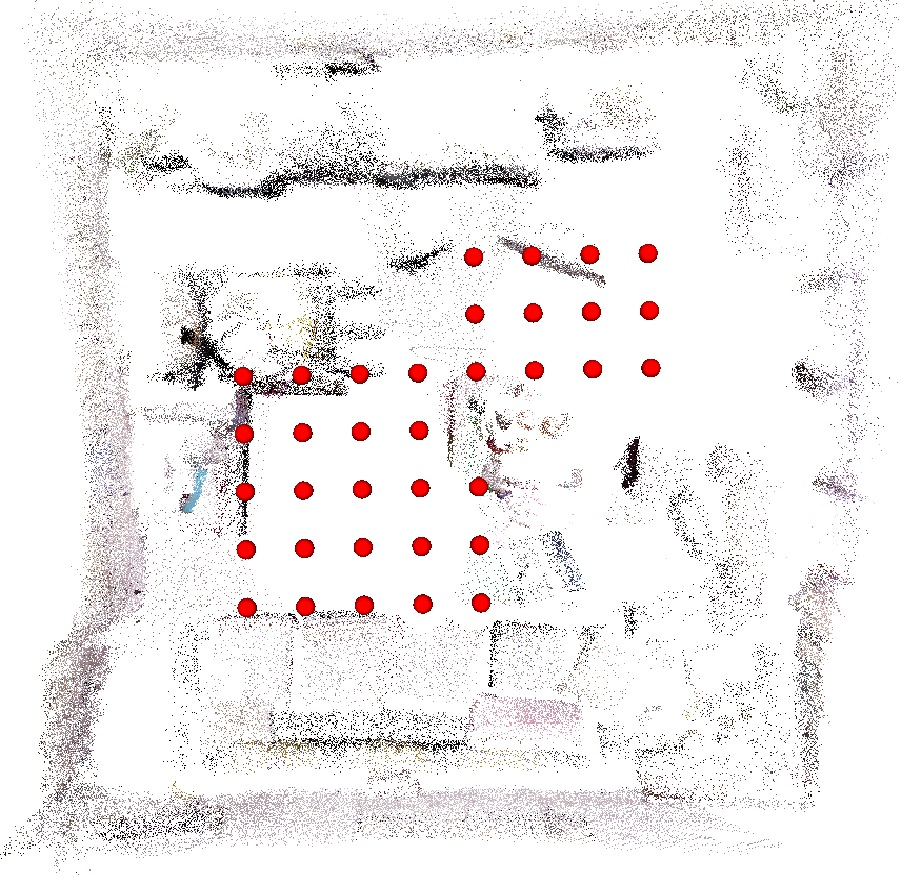
\includegraphics[width=0.4\columnwidth]{figures/LivingRoom_QueryPose.jpg}}
    \subfigure[定位環境 2.廚房 待定位照片分布位置]{\label{fig:Indoor_EV2_query}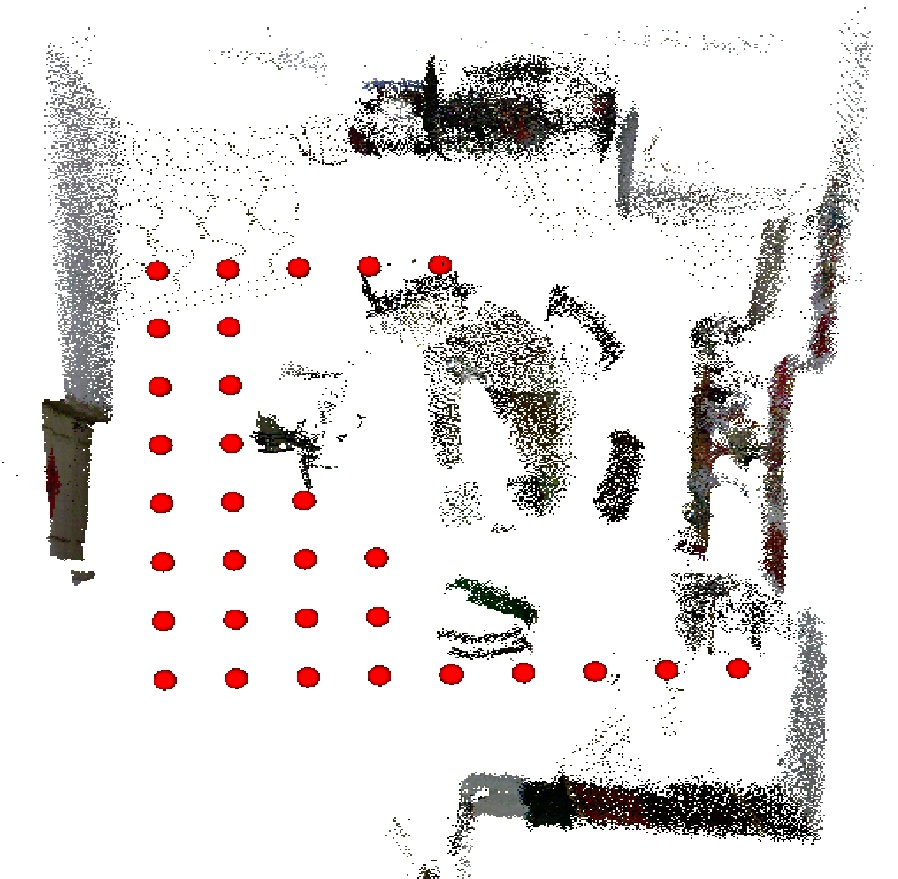
\includegraphics[width=0.4\columnwidth]{figures/Kitchen_QueryPose.jpg}}
	\end{center}
  \caption{室內定位環境與待定位照片分布位置}
  \label{fig:Indoor_EV_and_Query}	
\end{figure}		

\begin{figure}
	\begin{center}
	{\rotatebox{90}{
		\subfigure[客廳環境]{\label{fig:LivingRoom_Result}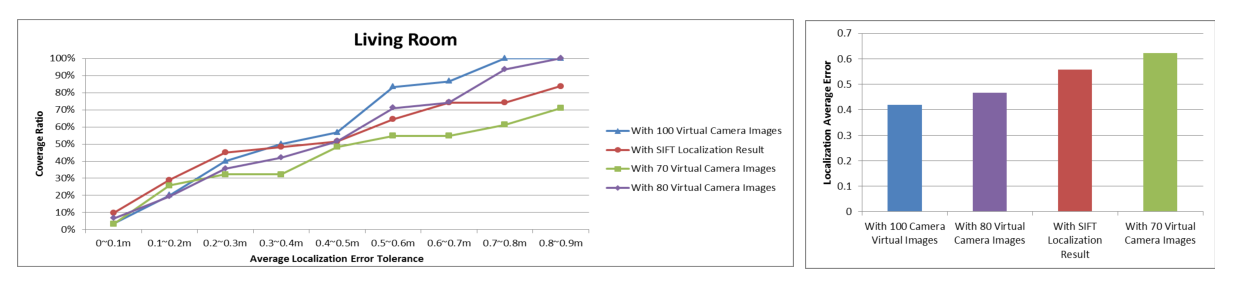
\includegraphics[width=1.2\columnwidth]{figures/Indoor_LivingRoom_Result.eps}}
		}
		\rotatebox{90}{
		\subfigure[廚房環境]{\label{fig:Kitchen_Result}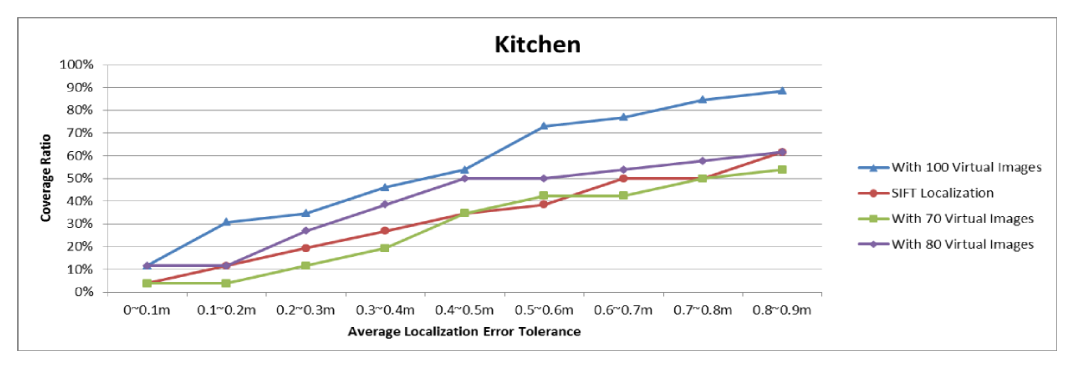
\includegraphics[width=1.2\columnwidth]{figures/Indoor_Kitchen_Result.eps}}
		}
		%\subfigure[平均定位誤差]{\label{fig:Indoor_EV2}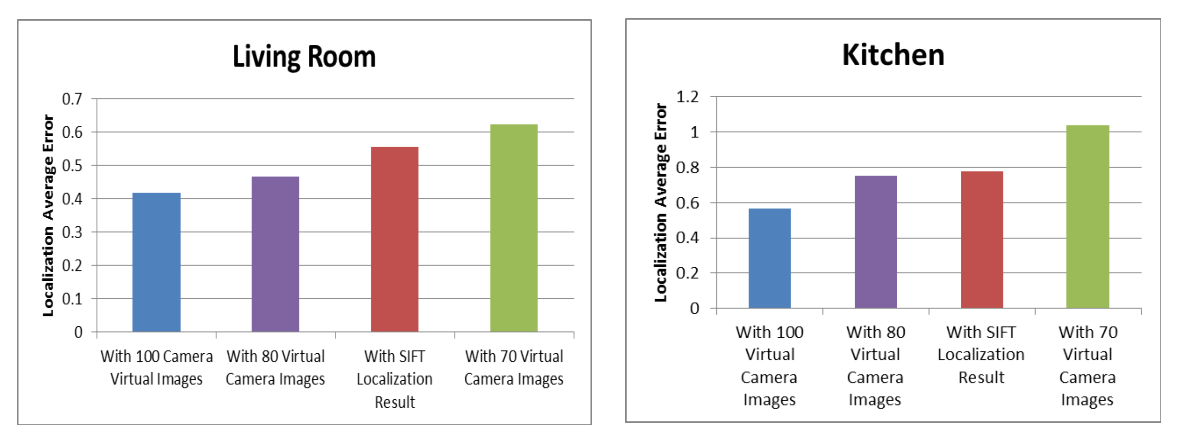
\includegraphics[width=1.0\columnwidth]{figures/Indoor_Average_Result.eps}}
		}
	\end{center}
  \caption{室內環境定位成果,上圖為誤差容忍範圍下定位成功覆蓋率,在容忍範圍下覆蓋率分布的變化,(a)為客廳環境,(b)為廚房環境}
  \label{fig:Indoor_EV_and_Query}	
\end{figure}	

\begin{figure}
\begin{center}
  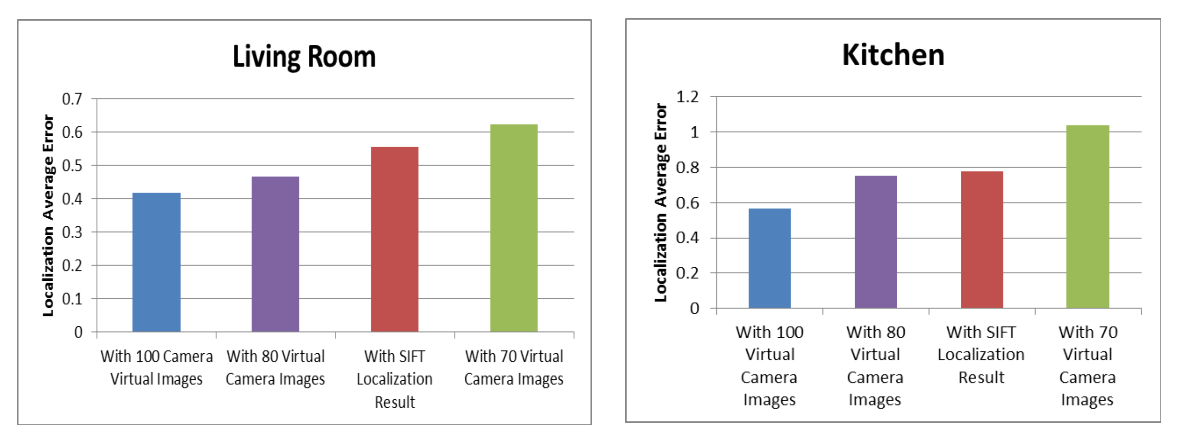
\includegraphics[width=1.0\textwidth]{figures/Indoor_Average_Result.eps}
  \caption{控制環境下定位平均誤差}
  \label{fig:Indoor_AVG_Error}
\end{center}
\end{figure}

		在室內定位的環境下,特徵點分布的數量,以及環境內觀測物的不同對定位結果增加許多變動因素。為了使定位結果能夠量化比較,我們將實驗結果分成(1).定位精準度
	覆蓋率,與(2).平均定位誤差兩個指標來分析成果。在圖\ref{fig:Indoor_EV_and_Query}之中來看,橫坐標表示定位誤差的容忍範圍,縱座標代表在這個誤差
	範圍下的定位成功率,以三種不同虛擬照片的數量與傳統2D影像照片做實驗比較。
	
		以覆蓋率來看,100張虛擬照片的定位結果為最好,代表取得越多點雲環境的資料,定位的改善越明顯。因為在每個相機位置上,我們取出兩張虛擬照片,所以在環境中總共有
	50個虛擬相機位置作比較,分別與40個與35個相機位置相比,有更多定位參考的依據。則平面2D影像因為只有一部分的環境參考依據,所以在定位覆蓋率與平均誤差,都比100張與
	80張虛擬照片定位成果來的差。以\ref{fig:LivingRoom_Result}來看,誤差範圍在$0.5m \sim 0.6m$之間的覆蓋率,以100張虛擬照片覆蓋率最高,有$80\%$左右的定位成功率,但是平面
	2D影像只有$60\%$左右的成功率,增加了$20\%$的覆蓋率。
	
		以平均誤差來說也有改善,在上個章節中我們發現平面2D影像定位誤差會有不穩定的情況發生,這種情況增加了整
	體的平均定位誤差,而在虛擬影像定位因為誤差會穩定在$1m$以內的範圍內,所以也會降低平均定位誤差。在圖\ref{fig:Indoor_AVG_Error}來看,室內環境下的平均定位誤差也獲得改善,而大多
	的平均誤差都可控制到0.5 m以下,以虛擬影像的平均定位誤差來說,與平面影像定位相比,當大於40組虛擬相機位置時,都可以改善平均定位誤差。
	
		從兩個定位環境下以圖\ref{fig:Indoor_EV1_query}與圖\ref{fig:Indoor_EV2_query}分別看兩個待定位圖片分布的情形,得知在廚房的環境的待定位圖片分布偏向於同一側,
	另一側因為障礙物阻擋,對於實際相機取得較為困難。因為平面影像定位的環境資料缺乏,導致定位誤差上升,尤其以兩個定位環境互相比對最為明顯。但整體來說,100張虛擬影像所取得定位
	成果都最為穩定,說明虛擬影像可以在一定的數量下可以補足環境資訊的缺乏,藉由優化相機角度增加影像的相關性,在相機無法拍攝的位置取得影像及避開障礙物,使得整體覆蓋率與誤差都能
	改善。

